\section{Experiments}\label{sec:exp}
\subsection{Implementation Details}
% Source: configs/lecun-deliver_rgbdel_P46_c3only_seed20260821_screen40_A2hires.yaml (TRAIN, OPTIMIZER, SCHEDULER, LOSS, MODEL.M2F, MODEL.P46.C3_PROTO, MODEL.P39).
All sensors are converted to three-channel images as in CMNeXt~\cite{cmnext2023}. We train for 40 epochs with AdamW (learning rate $6\times10^{-4}$, weight decay 0.01), a polynomial schedule with power 0.9, and a 10-epoch warm-up, on $768\times768$ crops with an effective batch size of 16 obtained by gradient accumulation. We use the data augmentation of DGFusion~\cite{dgfusion2026} so that both models see the same augmented images. The segmentation loss combines online hard-example cross-entropy~\cite{ohem2016} on the dense head with the set-prediction loss of the query head (weight 0.5, with deep supervision) and three auxiliary terms inherited from earlier versions of our model: an auxiliary cross-entropy on the fusion output, a class-prototype contrastive term (weight 0.1), and a variance-covariance regularizer on the fused tokens; we list them for reproducibility and do not claim them as contributions \todo{one-line ablation or citation for the auxiliary terms, or move to the supplement}. The frozen teacher is the same architecture without the high-resolution path, trained for 200 epochs on clean data. Unless noted, we report the mean of three seeds and the best seed; ablations use one seed.

\subsection{Comparison with Prior Fusion Models}
Table~\ref{tab:deliver} compares \ours{} with fusion models on DELIVER. We list only methods evaluated under the protocol that reports test-split mIoU, because DELIVER results in the literature are reported under at least three different protocols and are not comparable across them. \ours{} reaches 57.74 test mIoU on average over three seeds and 58.61 for the best seed, 1.0 and 1.9 points above DGFusion. Its margin over MM SAM-adapter, which uses only RGB and depth, is 0.4 points on average \todo{val 3-seed mean; val comparison with CAFuser-CAA 68.79}. Tables~\ref{tab:muses} and~\ref{tab:mcubes} report the same model on the real MUSES and MCubeS benchmarks \todo{results pending: MUSES four-sensor model, MCubeS transfer}.
% Sources: headline.yaml deliver.ours[0] (57.74 / best 58.61; gap +1.03 / +1.90 vs DGFusion 56.71; +0.39 / +1.26 vs MM SAM-adapter 57.35);
% protocol clusters: repo research/novelty-and-related-work.md l.74-85 (secondary; cite original tables).


% Layout rule (user 2026-10-27): no \resizebox on tables. Every table uses \tabsetup and
% tabular* at \columnwidth, so all tables share one font size and none overflows the column.

% ---------------------------------------------------------------------------
% Table 1. DELIVER, all four sensors.
% Baselines: only the test-unified cluster (DGFusion protocol, "mIoU-test").
%   Do NOT mix with the high cluster (CMNeXt 66.30 / MemorySAM 65.38).
%   Candidate values for todo cells are in repo research/novelty-and-related-work.md:78-83
%   (secondary copy) -> must be taken from each original paper table, cite table+page.
% Ours: experiments/headline.yaml benchmarks.deliver.ours[0] (A2, 3 seeds, legal v2, test@1024).
%   val 3-seed mean is not recorded in headline.yaml (only seed903 69.86) -> todo.
% ---------------------------------------------------------------------------
\begin{table}[t]
\caption{DELIVER (RGB, depth, event, LiDAR), mIoU (\%).}
\label{tab:deliver}
\centering\tabsetup
\begin{tabular*}{\columnwidth}{@{\extracolsep{\fill}}lllcc@{}}
\toprule
Method & Backbone & Sensors & val & test \\
\midrule
CMNeXt~\td & \td & RGB-D-E-L & \td & \td \\
StitchFusion~\td & \td & RGB-D-E-L & \td & \td \\
GeminiFusion~\td & \td & RGB-D-E-L & \td & \td \\
CAFuser~\td & \td & RGB-D-E-L & \td & \td \\
CAFuser-CAA~\td & \td & RGB-D-E-L & 68.79 & \td \\
DGFusion~\td & Swin-T & RGB-D-E-L & \td & 56.71 \\
\midrule
\multicolumn{5}{@{}l}{\emph{Fewer sensors (secondary comparison)}} \\
MM SAM-adapter~\td & \td & RGB-D & 69.60 & 57.35 \\
\midrule
Ours (3-seed mean) & DINOv3-L & RGB-D-E-L & \td & 57.74 \\
Ours (best seed) & DINOv3-L & RGB-D-E-L & \td & 58.61 \\
\bottomrule
\end{tabular*}
\tabnote{\textcolor{red}{todo: original table/page per baseline; protocol (val-best checkpoint, 1024, nearest-exact label resampling); DINOv3-L is frozen.}}
\end{table}

% ---------------------------------------------------------------------------
% Table 2. MUSES, four sensors (RGB, event, LiDAR, radar). Only the 4-sensor A2 model
%   (user 2026-09-29; 3-sensor numbers 79.788 etc. are not used).
% Ours: DRN-261019-02 (queued) -> todo. Baselines: headline.yaml benchmarks.muses.
% ---------------------------------------------------------------------------
\begin{table}[t]
\caption{MUSES, official evaluation, mIoU (\%).}
\label{tab:muses}
\centering\tabsetup
\begin{tabular*}{\columnwidth}{@{\extracolsep{\fill}}lllcc@{}}
\toprule
Method & Backbone & Sensors & val & test \\
\midrule
CAFuser~\td & \td & \td & \td & \td \\
DGFusion~\td & \td & \td & \td & 79.5 \\
\midrule
\multicolumn{5}{@{}l}{\emph{Camera only or fewer sensors (secondary comparison)}} \\
GtA~\td & \td & RGB & \td & 82.39 \\
MM SAM-adapter~\td & \td & RGB-L & \td & 81.07 \\
\midrule
Ours & DINOv3-L & RGB-E-L-R & \td & \td \\
\bottomrule
\end{tabular*}
\end{table}

% ---------------------------------------------------------------------------
% Table 3. MCubeS (RGB, AoLP, DoLP, NIR). Ours: DRN-261017-02 (A2 transfer, 2 seeds) -> todo.
%   58.07 in headline.yaml is the previous generation (P39.1 recipe), not the paper model.
% ---------------------------------------------------------------------------
\begin{table}[t]
\caption{MCubeS (RGB, AoLP, DoLP, NIR), test mIoU (\%).}
\label{tab:mcubes}
\centering\tabsetup
\begin{tabular*}{\columnwidth}{@{\extracolsep{\fill}}llc@{}}
\toprule
Method & Backbone & test \\
\midrule
Mul-VMamba~\td & \td & 54.65 \\
StitchFusion~\td & \td & 55.9 \\
\midrule
Ours & DINOv3-L & \td \\
\bottomrule
\end{tabular*}
\end{table}

\subsection{Robustness to Missing and Degraded Sensors}
Table~\ref{tab:robust} and Fig.~\ref{fig:robust} evaluate all models under the same missing-sensor and noise protocol. Under the public benchmark definition on the validation set, \ours{} scores 57.85 EMM, 7.9 points above the best published result, and it keeps 61 to 66 mIoU when a quarter to three quarters of a sensor's pixels are missing. On the test set, the official DGFusion weights fall to 31.5 EMM and to 5.5 mIoU under the strongest noise, which shows how much the accuracy-oriented models depend on complete inputs. Re-training DGFusion and CAFuser with our synthetic degradation raises their EMM to 45.5 and 46.5 without changing their architecture. \ours{} reaches 48.7 EMM while keeping the highest clean accuracy, so it does not trade accuracy for robustness, and it retains 47.9 mIoU under the strongest noise, which was never seen during training.
% Sources: tasks/DRN-261019-03/analysis.md (val EMM15 57.85, RMM 65.53/63.35/61.28, test EMM15 48.66, NM 47.85);
% judgment-ledger 2026-10-01 row (DGFusion (a) EMM 31.53, NM .20 5.52; (b) EMM 45.52); current.md (4) CAFuser (b) EMM 46.50.

When only one sensor is available (Fig.~\ref{fig:robust}b), the official DGFusion collapses to 12.1 mIoU with RGB alone and to 1.2 and 3.2 with event or LiDAR alone, while still reaching 43.1 with depth alone. Training with degraded inputs lifts every single-sensor score, most strongly for RGB (49.0 for the re-trained DGFusion and 53.9 for our model without the high-resolution path). Sensor dependence, in other words, follows the training data.
% Source: judgment-ledger 2026-10-01 row (single-sensor EMM subsets; Q2 3 seeds 53.9/46.0/31.0/22.9).

% ---------------------------------------------------------------------------
% Table 4. Missing and degraded sensors on DELIVER.
% (a) Benchmark family (2503.18445 definition: normalize then zero-fill), val.
%     Ours: tasks/DRN-261019-03/analysis.md (A2 3 seeds, mm_eval_v2): EMM15 57.85,
%     RMM15 r.25/.5/.75 65.53/63.35/61.28. RMMSS EMM 49.93: same doc / headline.yaml note.
% (b) Same protocol, our measurement on test (61 cases, 1897 images):
%     DGFusion (a) official weights / (b) degradation retrained: experiments/judgment-ledger.md
%       2026-10-01 row (DRN-260930-02). CAFuser (b): status/current.md (4) "CAFuser (b) 10-04".
%     "w/o two-pass" = E1 40ep screen 3 seeds, EMM 40.01: ledger 2026-10-01 row.
%     "w/o high-res" = Q2 3 seeds, "Ours" = A2 3 seeds: tasks/DRN-261019-03/analysis.md
%       (Q2 NM is 2 seeds for s902/s903 plus s821 where available; see that table).
%     Depth/RGB partial-drop columns omitted: Q2 values disagree between ledger 10-01 (3 seeds:
%     0.98/2.04/2.64) and DRN-261019-03 (2 seeds: 0.47/1.05/1.36) -> resolve before use.
% Families that skip missing inputs (AnySeg, RMMSS, RobustSeg 1a, FuseAdapt) are not mixed here.
% ---------------------------------------------------------------------------
\begin{table}[t]
\caption{Robustness to missing and degraded sensors on DELIVER, mIoU (\%).}
\label{tab:robust}
\centering\tabsetup
\begin{tabular*}{\columnwidth}{@{\extracolsep{\fill}}lccccc@{}}
\toprule
\multicolumn{6}{@{}l}{\emph{(a) Public missing-modality benchmark, val}} \\
Method & EMM & RMM .25 & RMM .50 & RMM .75 & \\
\midrule
RMMSS~\td & 49.93 & \td & \td & \td & \\
Ours (3 seeds) & 57.85 & 65.53 & 63.35 & 61.28 & \\
\midrule
\multicolumn{6}{@{}l}{\emph{(b) Same protocol for all models, test}} \\
Method & Clean & EMM & S\&P .05 & S\&P .10 & S\&P .20 \\
\midrule
DGFusion (official) & 55.68 & 31.53 & 37.97 & 16.71 & 5.52 \\
DGFusion (retrained$^{\dagger}$) & 54.77 & 45.52 & 48.89 & 40.51 & 23.34 \\
CAFuser (retrained$^{\dagger}$) & 55.79 & 46.50 & \td & \td & \td \\
Ours w/o two-pass & \td & 40.01 & \td & \td & \td \\
Ours w/o high-res & 56.59 & 48.06 & 53.25 & 51.64 & 48.79 \\
Ours & 57.74 & 48.66 & 53.11 & 51.36 & 47.85 \\
\bottomrule
\end{tabular*}
\tabnote{$^{\dagger}$Retrained with the same synthetic degradation. Ours: mean of 3 seeds; baselines: single runs.
\textcolor{red}{todo: define EMM (mean over 15 sensor subsets), RMM (random drop ratio), S\&P noise.}}
\end{table}

% ---------------------------------------------------------------------------
% Fig. robust (data plot). Source numbers and provenance: figures/src/make_data_figs.py (fig_robust).
% ---------------------------------------------------------------------------
\begin{figure}[t]
\centering
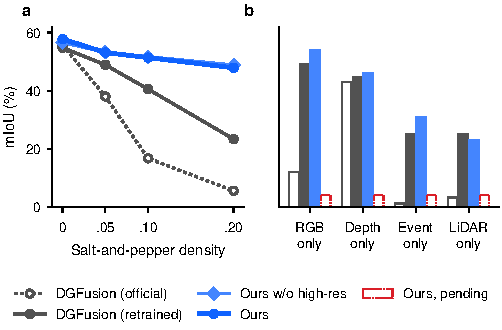
\includegraphics[width=\columnwidth]{figures/fig_robust.pdf}
\caption{Robustness on DELIVER test under one protocol. (a) Salt-and-pepper noise applied to every sensor. (b) Only one sensor available (the other three zero-filled). Ours: mean of three seeds; DGFusion: single runs, official weights or retrained with the same synthetic degradation. \todo{(b) full-model values pending.}}
\label{fig:robust}
\end{figure}

\subsection{Qualitative Results}
Figs.~\ref{fig:failure_scenarios} and~\ref{fig:adverse} show scenes selected by a fixed rule: among all test images, those where the gap between our model and the best baseline is largest, at most one scene per condition and map \todo{describe what the scenes show once selected}.

% Fig. sensor-failure scenarios (main qualitative figure). Needs per-image predictions of
% DGFusion (official), DGFusion/CAFuser (retrained) and ours under missing/noisy sensors
% -> analysis request inbox 20261027-182054 item 2.
\begin{figure*}[t]
\centering
\phbox{5.2cm}{Fig.~3 when a sensor fails: rows = depth missing / RGB missing / LiDAR+event missing / RGB with heavy noise; columns = affected input, ground truth, DGFusion (official), DGFusion (retrained), CAFuser (retrained), ours; error pixels in one colour}
\caption{\todo{caption; state the scene-selection rule (top differences between ours and the best baseline, one scene per condition, no repeated map)}}
\label{fig:failure_scenarios}
\end{figure*}

% Fig. adverse conditions with all sensors present, DELIVER (synthetic) + MUSES (real).
% DELIVER dumps exist: NAS analysis_logs/native_axis_baseline_20261016/{dgfusion,cafuserb}_test1024,
% a2_test1024_dump_20261016/s821 -> analysis request inbox 20261027-182054 item 1. MUSES: item 3.
\begin{figure*}[t]
\centering
\phbox{4.6cm}{Fig.~4 adverse conditions, all sensors present: DELIVER night / fog / rain / low exposure and MUSES real night / snow / fog; columns = RGB, ground truth, DGFusion, CAFuser, ours; zoomed crops where the baselines miss objects}
\caption{\todo{caption; state the scene-selection rule}}
\label{fig:adverse}
\end{figure*}

\subsection{Accuracy per Condition}
Table~\ref{tab:condition} breaks clean test accuracy down by condition \todo{text after the per-condition numbers arrive (analysis request 20261028-183826 item 1)}.

% ---------------------------------------------------------------------------
% Table 5. Clean mIoU per condition on DELIVER test (new 2026-10-28, user: 10-page budget).
% Source: to be computed by analysis from the same dumps as Fig. adverse (inbox addendum).
% ---------------------------------------------------------------------------
\begin{table}[t]
\caption{DELIVER test mIoU (\%) per condition, all sensors present.}
\label{tab:condition}
\centering\tabsetup
\begin{tabular*}{\columnwidth}{@{\extracolsep{\fill}}lccccccc@{}}
\toprule
Model & Sun & Cloud & Rain & Fog & Night & Low exp. & All \\
\midrule
DGFusion (official) & \td & \td & \td & \td & \td & \td & 55.68 \\
DGFusion (retrained$^{\dagger}$) & \td & \td & \td & \td & \td & \td & 54.77 \\
CAFuser (retrained$^{\dagger}$) & \td & \td & \td & \td & \td & \td & 55.79 \\
Ours w/o high-res & \td & \td & \td & \td & \td & \td & 56.59 \\
Ours & \td & \td & \td & \td & \td & \td & 57.74 \\
\bottomrule
\end{tabular*}
\tabnote{$^{\dagger}$Retrained with synthetic degradation. All: same values as Table~\ref{tab:robust}(b) clean column.}
\end{table}

\subsection{Ablation}
Table~\ref{tab:ablation} builds the model up from a frozen DINOv3-L with LoRA on RGB alone and then removes one component at a time from the full model, all with the same seed and schedule. The frozen backbone alone reaches 55.14 mIoU with RGB, already within 1.6 points of DGFusion with four sensors, so a large part of the accuracy comes from the foundation model. Adding the other three sensors with cross-modal attention and the query head gives 55.94, the two-pass training with distillation adds 1.8 points (57.73), and the high-resolution path adds 0.9 (58.61). Removing cross-modal attention or the query head costs 0.85 and 0.72 points, respectively. Replacing the sensor-specific adapters with one shared adapter does not reduce clean accuracy (58.84) \todo{robustness of the shared variant and the degradation-pass and distillation rows (L5, L6) pending}.
% Sources: judgment-ledger 2026-10-28 rows DRN-261020-08/-09/-10/-12 (seed 821, legal v2 test@1024);
% E1 screen s821 55.94: status/current.md (4); Q2/A2 s821 57.73/58.61: tasks/DRN-261019-03/analysis.md.

% ---------------------------------------------------------------------------
% Table 6. Ablation on DELIVER test, seed 821, 40 epochs, legal v2.
% RGB-only 55.14 = judgment-ledger 2026-10-28 DRN-261020-08 (adopted as ladder row).
% L1 shared LoRA 58.84, L2 mean fusion 57.76, L4 dense head only 57.89 = judgment-ledger 2026-10-28
%   rows DRN-261020-09/-10/-12 (test@1024 legal v2, seed 821). L2 also removes the trunk expansion
%   (code constraint, ledger note). L5 DRN-261020-13 / L6 -14 evaluating; mean-fusion ladder -07 running.
% mean fusion = DRN-261020-07 (evaluating). E1 screen s821 55.94 = status/current.md (4).
% Q2 s821 57.73 / EMM 48.68 and A2 s821 58.61 / EMM 49.12 = tasks/DRN-261019-03/analysis.md.
% Leave-one-out: L1 DRN-261020-09, L2 -10, L4 -12, L5 -13, L6 -14 (queued). L3 withdrawn.
% ---------------------------------------------------------------------------
\begin{table}[t]
\caption{Ablation on DELIVER test (one seed, 40 epochs), mIoU (\%).}
\label{tab:ablation}
\centering\tabsetup
\begin{tabular*}{\columnwidth}{@{\extracolsep{\fill}}lcc@{}}
\toprule
Configuration & Clean & EMM \\
\midrule
\multicolumn{3}{@{}l}{\emph{Building up}} \\
Frozen DINOv3-L + LoRA, RGB only & 55.14 & -- \\
+ depth, event, LiDAR (mean fusion) & \td & \td \\
+ cross-modal attention, query head & 55.94 & \td \\
+ two-pass training, distillation & 57.73 & 48.68 \\
+ high-res path (full model) & 58.61 & 49.12 \\
\midrule
\multicolumn{3}{@{}l}{\emph{Removing one component from the full model}} \\
$-$ sensor-specific LoRA (one shared) & 58.84 & \td \\
$-$ cross-modal attention (mean fusion)$^{*}$ & 57.76 & \td \\
$-$ query head and arbiter & 57.89 & \td \\
$-$ degradation pass & \td & \td \\
$-$ teacher distillation & \td & \td \\
\bottomrule
\end{tabular*}
\tabnote{$^{*}$Also removes the trunk expansion. \textcolor{red}{todo: EMM column for ablation runs; decision on shared LoRA pending its robustness test.}}
\end{table}

\subsection{Computational Cost}
Table~\ref{tab:cost} reports parameters, operations, latency, and memory at the evaluation resolution \todo{numbers pending (DRN-261027-02); the two-pass training doubles the forward passes during training but adds nothing at inference}.

% ---------------------------------------------------------------------------
% Table 7. Cost on DELIVER at 1024, same GPU. DRN-261027-02 (queued) -> all todo.
% ---------------------------------------------------------------------------
\begin{table}[t]
\caption{Computational cost on DELIVER at $1024\times1024$.}
\label{tab:cost}
\centering\tabsetup
\begin{tabular*}{\columnwidth}{@{\extracolsep{\fill}}lccccc@{}}
\toprule
Model & Params & Trainable & GFLOPs & Latency & Memory \\
 & (M) & (M) & & (ms) & (GB) \\
\midrule
DGFusion & \td & \td & \td & \td & \td \\
CAFuser & \td & \td & \td & \td & \td \\
Ours w/o high-res & \td & \td & \td & \td & \td \\
Ours & \td & \td & \td & \td & \td \\
\bottomrule
\end{tabular*}
\end{table}
